\documentclass{beamer}
%\documentclass[xcolor=dvipsnames]{beamer}
\usepackage[spanish]{babel}
\usepackage[utf8]{inputenc}
\usepackage{graphicx}
\usepackage{hyperref}
\usepackage{breakurl}

\newcommand{\beamer}{\textsc{beamer}}
\newtheorem{definicion}{Definición}
\newtheorem{ejemplo}{Ejemplo}

%%%%%%%%%%%%%%%%%%%%%%%%%%%%%%%%%%%%%%%%%%%%%%%%%%%%%%%%%%%%%%%%%%%%%%%%%%%%%%%
\title[Defensa Oral TFG]{Análisis de los resultados de los sistemas de entrenamiento del Pensamiento Computacional}
\subtitle{Analysis of the results of Computational Thinking training systems}
\author[Samuel Valcárcel Arce]{Autor: Samuel Valcárcel Arce \\ Tutora: Coromoto León Hernández}
\institute[ULL]{Universidad de La Laguna}
\date[\today]{\today}
%%%%%%%%%%%%%%%%%%%%%%%%%%%%%%%%%%%%%%%%%%%%%%%%%%%%%%%%%%%%%%%%%%%%%%%%%%%%%%%

\usetheme{Madrid}
%\usetheme{Warsaw}

%%%%%%%%%%%%%%%%%%%%%%%%%%%%%%%%%%%%%%%%%%%%%%%%%%%%%%%%%%%%%%%%%%%%%%%%%%%%%%%
\definecolor{pantone254}{RGB}{91,19,138}
\definecolor{pantone3015}{RGB}{0,88,147}
\definecolor{pantone432}{RGB}{56,61,66}
\setbeamercolor*{palette primary}{use=structure,fg=white,bg=pantone254}
\setbeamercolor*{palette secondary}{use=structure,fg=white,bg=pantone3015}
\setbeamercolor*{palette tertiary}{use=structure,fg=white,bg=pantone432}
\setbeamercolor*{palette sidebar primary}{use=structure,fg=pantone254}
\setbeamercolor*{palette sidebar tertiary}{use=structure,fg=pantone3015}
\setbeamercolor*{block title}{bg=pantone3015,fg=white}
\setbeamercolor*{alerted text}{fg=pantone432}
\setbeamercolor*{item projected}{fg=pantone254}
\setbeamercolor*{section in toc shaded}{use=structure,fg=structure.fg}
\setbeamercolor*{section in toc}{fg=pantone3015}
\setbeamercolor*{subsection in toc shaded}{fg=pantone3015}
\setbeamercolor*{subsection in toc}{fg=pantone432}

%%%%%%%%%%%%%%%%%%%%%%%%%%%%%%%%%%%%%%%%%%%%%%%%%%%%%%%%%%%%%%%%%%%%%%%%%%%%%%%
\begin{document}
  
%++++++++++++++++++++++++++++++++++++++++++++++++++++++++++++++++++++++++++++++  
\begin{frame}
  \begin{figure}
  
\includegraphics[width=0.5\textwidth]{img/logo_nuevo.eps}
  \end{figure}
  \hspace*{7.5cm}
  \titlepage

\end{frame}
%++++++++++++++++++++++++++++++++++++++++++++++++++++++++++++++++++++++++++++++  

%++++++++++++++++++++++++++++++++++++++++++++++++++++++++++++++++++++++++++++++  
\begin{frame}
  \frametitle{Índice}  
  \tableofcontents[pausesections]
\end{frame}
%++++++++++++++++++++++++++++++++++++++++++++++++++++++++++++++++++++++++++++++  


\section{Motivación y Objetivos}


%++++++++++++++++++++++++++++++++++++++++++++++++++++++++++++++++++++++++++++++  
\begin{frame}

\frametitle{Motivación}

\begin{definicion}
Especificar la motivación del trabajo
\end{definicion}

\end{frame}
%++++++++++++++++++++++++++++++++++++++++++++++++++++++++++++++++++++++++++++++  

%++++++++++++++++++++++++++++++++++++++++++++++++++++++++++++++++++++++++++++++  
\begin{frame}

\frametitle{Objetivos }

\begin{block}{Ejemplo}
  \begin{itemize}
  \item
   Objetivo 1 
  \pause

  \item
   Objetivo 2

  \end{itemize}
\end{block}

\end{frame}
%++++++++++++++++++++++++++++++++++++++++++++++++++++++++++++++++++++++++++++++  

\section{Estado actual del arte}

\begin{frame}
\frametitle{Estado actual del arte}

Se presentarán los antecedentes teóricos y prácticos que apoyan el tema objeto
del trabajo.

\end{frame}
%++++++++++++++++++++++++++++++++++++++++++++++++++++++++++++++++++++++++++++++  

\section{Procedimiento experimental}

\begin{frame}
\frametitle{Procedimiento experimental}

Ha de contar con secciones para la descripción de los experimentos y del material.
También deber haber una sección para los resultados obtenidos y una última de
análisis de los resultados obtenidos.

\end{frame}
%++++++++++++++++++++++++++++++++++++++++++++++++++++++++++++++++++++++++++++++  

\subsection{Descripción de los experimentos}

%++++++++++++++++++++++++++++++++++++++++++++++++++++++++++++++++++++++++++++++  
\begin{frame}
\frametitle{Generación de datos aleatoria}

\begin{ejemplo}
  \begin{itemize}
    \item <1-> Con semilla 1 
    \item <2-> Con semilla 10 
    \item <3> Sin semilla 
  \end{itemize}
\end{ejemplo}

\end{frame}
%++++++++++++++++++++++++++++++++++++++++++++++++++++++++++++++++++++++++++++++  

\subsection{Descripción del material}
%++++++++++++++++++++++++++++++++++++++++++++++++++++++++++++++++++++++++++++++  
\begin{frame}
\frametitle{Hardware y Software}

\begin{ejemplo}
  \begin{enumerate}
    \item
      Descripción del hardware 
      \pause

    \item
      Descripción del software 
  \end{enumerate}
\end{ejemplo}

\end{frame}
%++++++++++++++++++++++++++++++++++++++++++++++++++++++++++++++++++++++++++++++  

\subsection{Resultados obtenidos}
%++++++++++++++++++++++++++++++++++++++++++++++++++++++++++++++++++++++++++++++  
\begin{frame}
\frametitle{Medidas de tiempo y Velocidad}

%------------------------------------------------------------------------------
%--------------------------------------------------------------------------
\begin{table}[!ht]
\begin{center}
\begin{tabular}{|p{60mm}|p{20mm}|p{40mm}|p{25mm}|} \hline 
\textbf{Recurso} & \textbf{Horas} & \textbf{Precio unidad} & \textbf{Total}\\ \hline
Estudio Pensamiento Computacional & 50 & 12\euro & 600\euro \\ \hline

Tutorial Ruby on Rails & 10 & 12\euro & 120\euro \\ \hline

Desarrollo de plataforma & 10 & 10\euro & 100\euro \\ \hline

Front-End & 50 & 12\euro & 600\euro \\ \hline

Back-End & 60 & 12\euro & 720\euro \\ \hline

Total & 170 & - &  \\ \hline

\end{tabular}
\end{center}
\caption{Tabla resumen del presupuesto}
\label{table:resOthers}
\end{table}

%------------------------------------------------------------------------------

\end{frame}
%++++++++++++++++++++++++++++++++++++++++++++++++++++++++++++++++++++++++++++++  


\subsection{Análisis de los resultados}
%++++++++++++++++++++++++++++++++++++++++++++++++++++++++++++++++++++++++++++++  
\begin{frame}
\frametitle{Diagrama del tiempo y la velocidad}

%------------------------------------------------------------------------------
\begin{figure}[!th]
\begin{center}
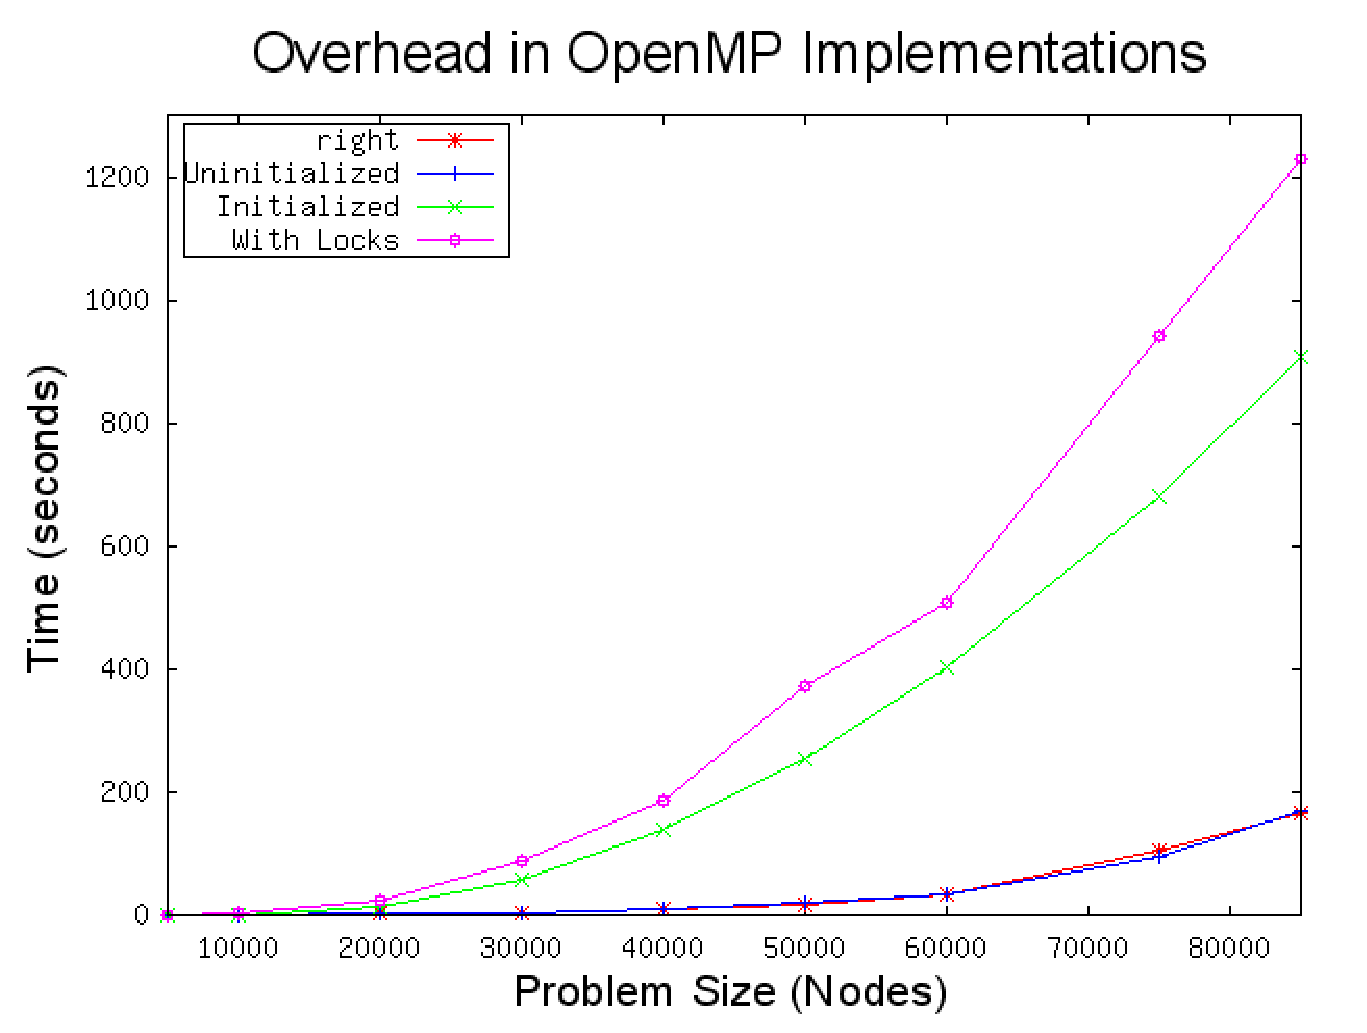
\includegraphics[width=0.75\textwidth]{img/figura1.eps}
\caption{Ejemplo de figura}
\label{fig:1}
\end{center}
\end{figure}
%------------------------------------------------------------------------------

\end{frame}
%++++++++++++++++++++++++++++++++++++++++++++++++++++++++++++++++++++++++++++++  


\section{Conclusiones}

%++++++++++++++++++++++++++++++++++++++++++++++++++++++++++++++++++++++++++++++  
\begin{frame}
\frametitle{Conclusiones}

\begin{ejemplo}
  \begin{enumerate}
    \item
      Conclusión 1
      \pause
    \item
      Conclusión 2
  \end{enumerate}
\end{ejemplo}

\end{frame}
%++++++++++++++++++++++++++++++++++++++++++++++++++++++++++++++++++++++++++++++  

%++++++++++++++++++++++++++++++++++++++++++++++++++++++++++++++++++++++++++++++  
\begin{frame}[allowframebreaks]
  \frametitle{Bibliografía}

  \begin{thebibliography}{10}

    \beamertemplatebookbibitems
    \bibitem[URL: Code.org]{latex} 
    Code.org. {\small{\url{https://code.org/}}}

    \beamertemplatebookbibitems
    \bibitem[URL: Hour of Code]{latex} 
    Hour of Code. {\small{\url{https://hourofcode.com/}}}

    \beamertemplatebookbibitems
    \bibitem[URL: Codecademy]{latex} 
    Codecademy. {\small{\url{https://www.codecademy.com/es}}}

    \beamertemplatebookbibitems
    \bibitem[URL: Programamos]{latex} 
    Programamos. {\small{\url{https://programamos.es/}}}

    \beamertemplatebookbibitems
    \bibitem[URL: Ruby on Rails]{latex} 
    Ruby on Rails. {\small{\url{https://rubyonrails.org/}}}

    \beamertemplatebookbibitems
    \bibitem[URL: Active Record Basics]{latex} 
    Active Record Basics. {\small{\url{http://guides.rubyonrails.org/active_record_basics.html}}}

    \beamertemplatebookbibitems
    \bibitem[URL: Bootstrap]{latex} 
    Bootstrap. {\small{\url{https://getbootstrap.com/}}}

    \beamertemplatebookbibitems
    \bibitem[URL: Chartkick]{latex} 
    Chartkick. {\small{\url{https://www.chartkick.com/}}}

    \beamertemplatebookbibitems
    \bibitem[URL: Github]{latex} 
    Github. {\small{\url{https://github.com/}}}

    \beamertemplatebookbibitems
    \bibitem[URL: RSpec]{latex} 
    RSpec. {\small{\url{http://rspec.info/}}}

    \beamertemplatebookbibitems
    \bibitem[URL: PuntoQ]{latex} 
    PuntoQ. {\small{\url{http://www.bbtk.ull.es/view/institucional/bbtk/Biblioteca_Digital/es}}}

    \beamertemplatebookbibitems
    \bibitem[URL: ACM]{latex} 
    ACM. {\small{\url{https://www.acm.org/publications/magazines}}}

    \beamertemplatebookbibitems
    \bibitem[URL: IEEE]{latex} 
    IEEE. {\small{\url{https://www.ieee.org/publications/periodicals.html}}}

    \beamertemplatebookbibitems
    \bibitem[URL: SQLite]{latex} 
    SQLite. {\small{\url{https://rubygems.org/gems/sqlite3/versions/1.3.11?locale=es}}}

    \beamertemplatebookbibitems
    \bibitem[URL: Devise]{latex} 
    Devise. {\small{\url{https://rubygems.org/gems/devise}}}

    \beamertemplatebookbibitems
    \bibitem[URL: Gem Bootstrap]{latex} 
    Gem Bootstrap. {\small{\url{https://rubygems.org/gems/bootstrap}}}

    \beamertemplatebookbibitems
    \bibitem[URL: Will-paginate]{latex} 
    Will-paginate. {\small{\url{https://rubygems.org/gems/will_paginate}}}

    \beamertemplatebookbibitems
    \bibitem[URL: Wicked-PDF]{latex} 
    Wicked-PDF. {\small{\url{https://rubygems.org/gems/wicked_pdf}}}

    \beamertemplatebookbibitems
    \bibitem[URL: Jquery-Rails]{latex} 
    Jquery-Rails. {\small{\url{https://rubygems.org/gems/jquery-rails}}}

    \beamertemplatebookbibitems
    \bibitem[Wilson, Cameron]{beamer} 
    Wilson, Cameron. 
    \emph{Hour of Code: Bringing Research to Scale} 
    {\small{\url{http://doi.acm.org.accedys2.bbtk.ull.es/10.1145/2746406}}}

    \beamertemplatebookbibitems
    \bibitem[M. Wing]{beamer} 
    M. Wing. 
    \emph{COMMUNICATIONS OF THE ACM March} 
    {\small{\url{https://www.cs.cmu.edu/{~}CompThink/papers/Wing06.pdf}}}

    \beamertemplatebookbibitems
    \bibitem[Tumlin, Nath]{beamer} 
    Tumlin, Nath. 
    \emph{Teacher Configurable Coding Challenges for Block Languages} 
    {\small{\url{http://doi.acm.org.accedys2.bbtk.ull.es/10.1145/3017680.3022467}}}

    \beamertemplatebookbibitems
    \bibitem[Brown, Neil C.C. and Monig, Jens and Bau, Anthony and Weintrop, David]{beamer} 
    Brown, Neil C.C. and Monig, Jens and Bau, Anthony and Weintrop, David. 
    \emph{Panel: Future Directions of Block-based Programming} 
    {\small{\url{http://doi.acm.org.accedys2.bbtk.ull.es/10.1145/2839509.2844661}}}


  \end{thebibliography}
\end{frame}


%++++++++++++++++++++++++++++++++++++++++++++++++++++++++++++++++++++++++++++++  

\end{document}
